The test environment considered is characterized by three corridors, divided by two curves, and has the following points of interest: the ADII classroom, the A28 classroom, a bathroom, a fire escape, an elevator, and a meeting room. To conduct the experiment and allow the algorithm implemented in the application to function correctly, several attempts were made to arrange the beacons in the considered section. 

In the final setting of the area, the beacons were placed at a distance of about 8 meters from each other and, in zones representing curves, they were placed at a slightly shorter distance to let the application be as responsive as possible in alerting the user of the presence of these particular regions. To permit easy identification of the points of interest, bands of several identical QR codes were attached to the floor at each of them and a QR code was affixed to the door or wall adjacent to it. 

\begin{figure*}
    \centering
    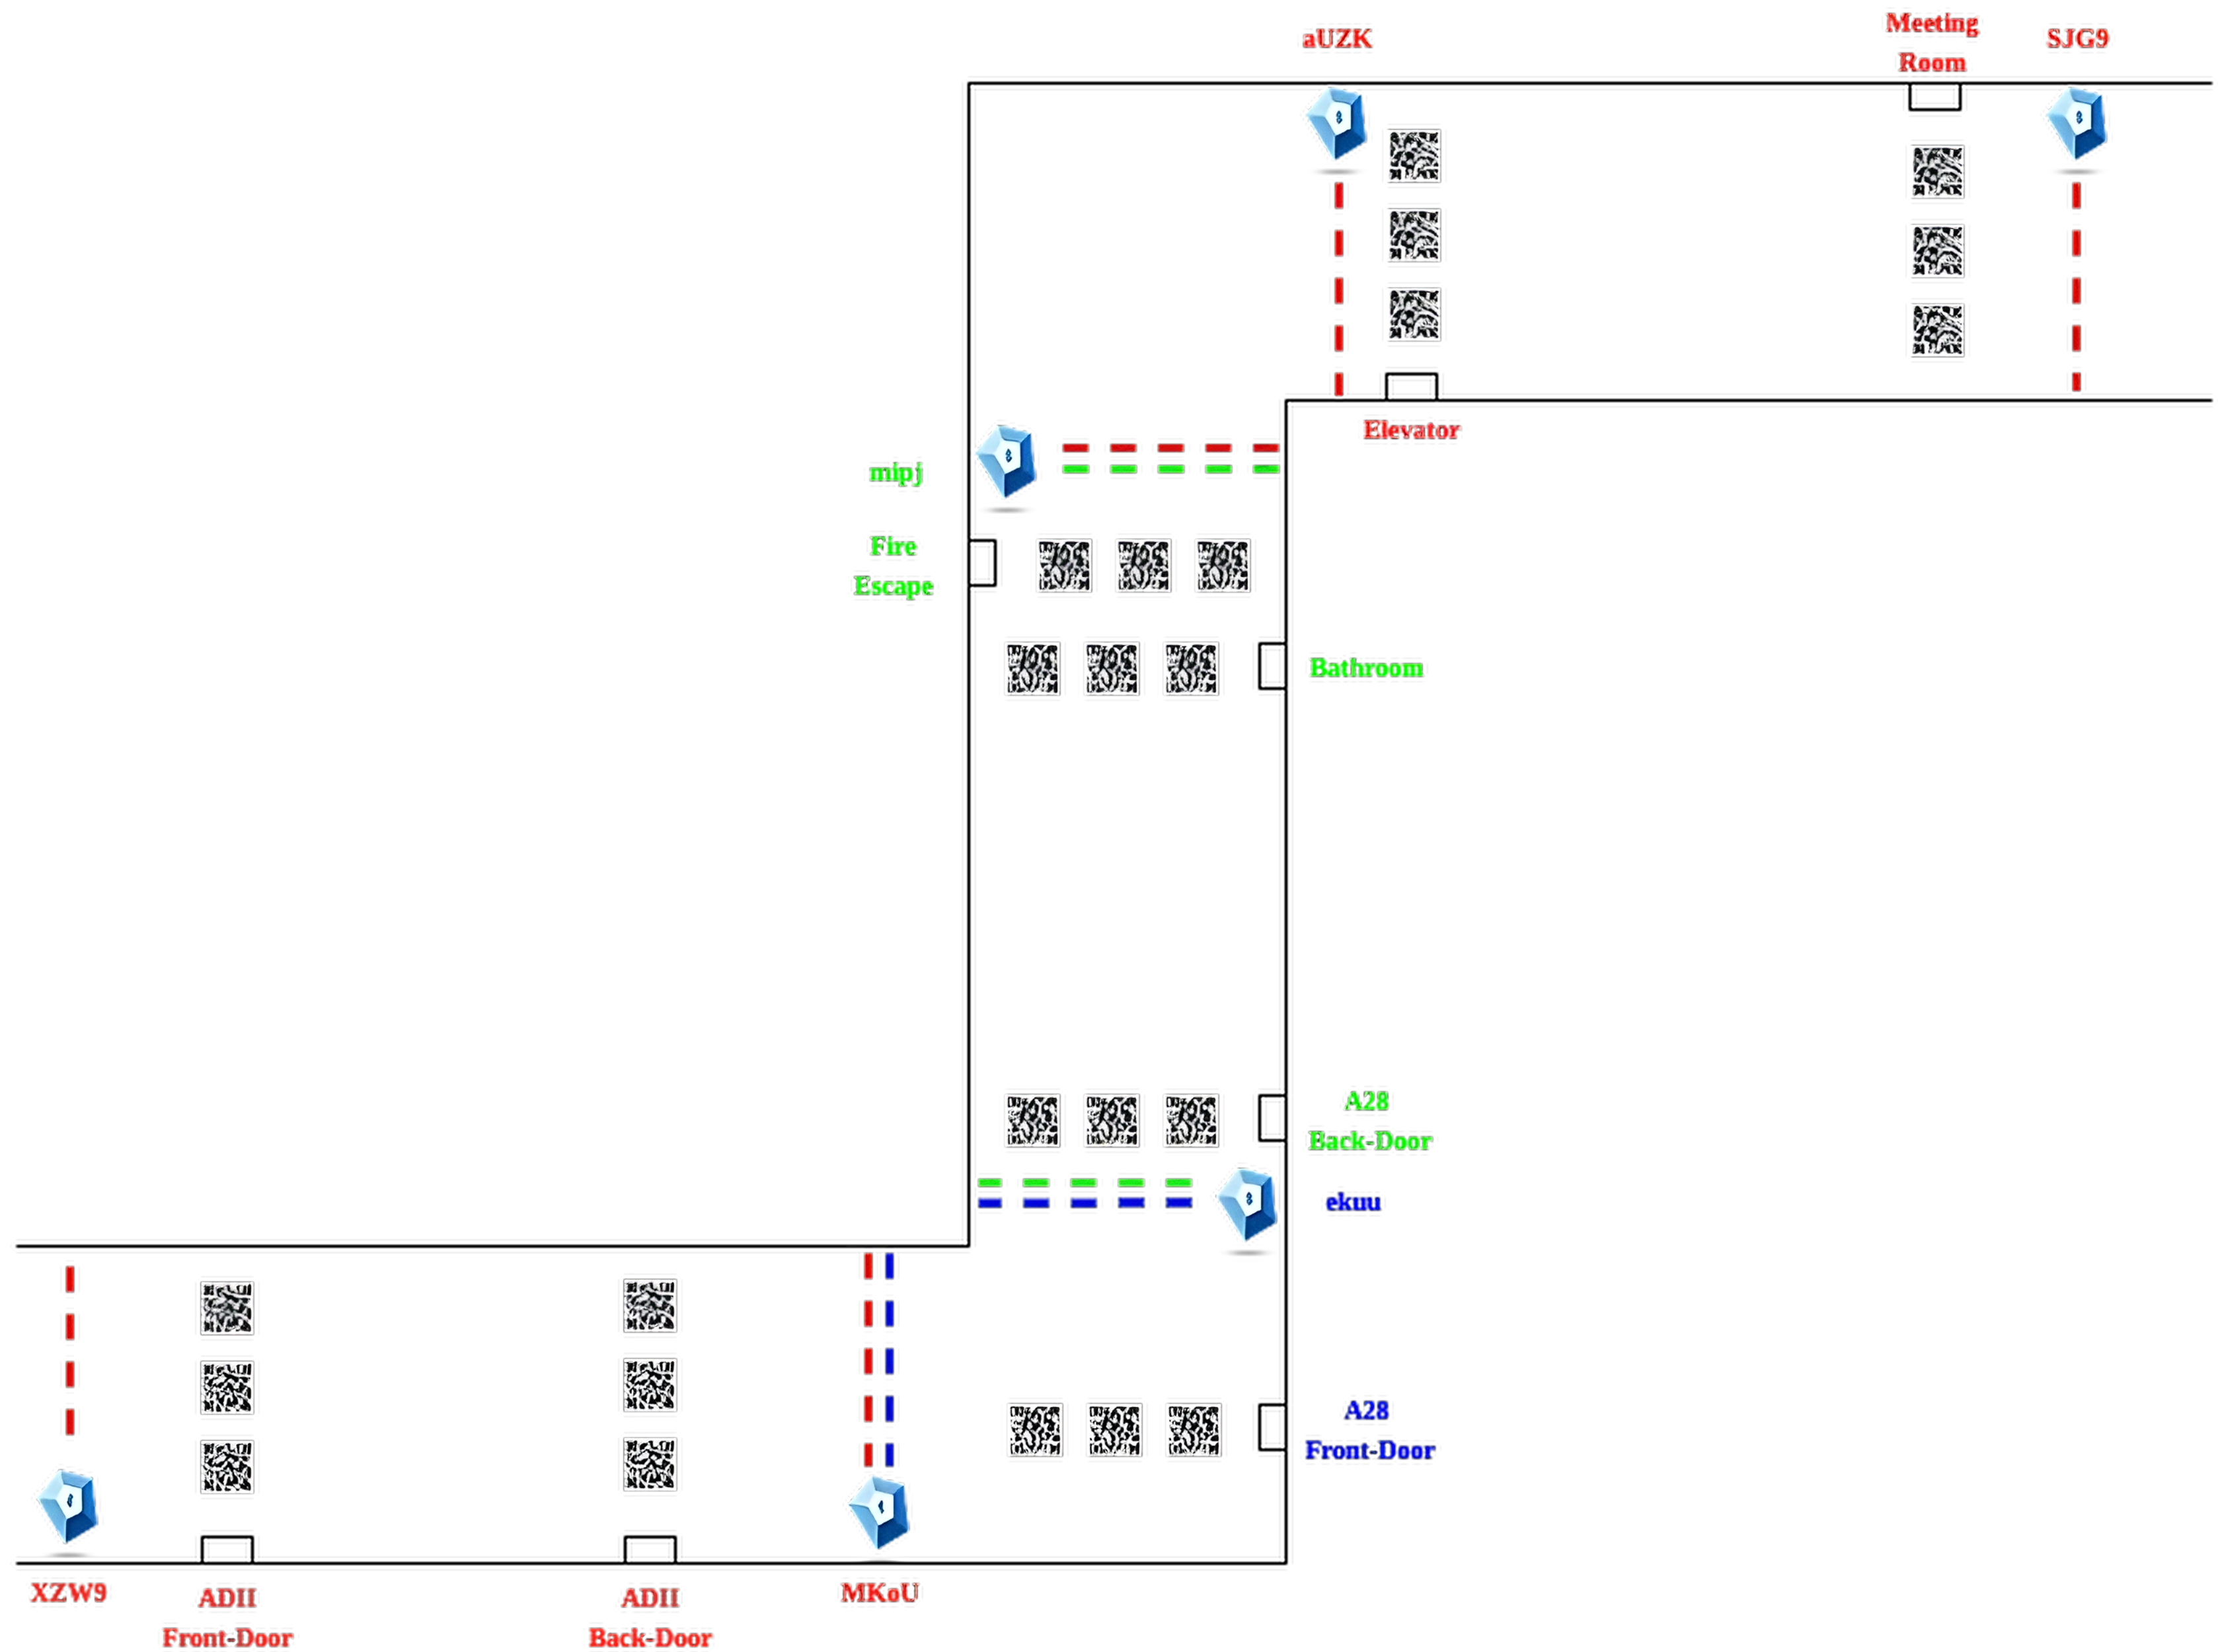
\includegraphics[scale = 0.12]{chapters/experimental_results/images/regions_mapping.png}
    \caption{Mapping of the regions and relative points of interest of the test area} 
    \label{fig:regions_mapping}
\end{figure*}
\noindent
Figure \ref{fig:regions_mapping} shows how the various initially introduced elements of the environment were mapped through the use of beacons and QR codes. This configuration was then placed into \textbf{JSON files} that are used by the application to be able to correctly execute the implemented detection algorithm.
